\section{Keypoint Selection}

In order to decide the keypoints detector we evaluate three methods: Harris, Shi-Tomasi (Good Features to Track) and SIFT (Scale Invariant Features). Figure \ref{fig:comparison-keypoints} shows some results for the feature extraction, we used OpenCV implementations for the detectors in this step.

\begin{figure}[!h]
	\centering
	\begin{subfigure}{0.5\textwidth}
	  \centering
	  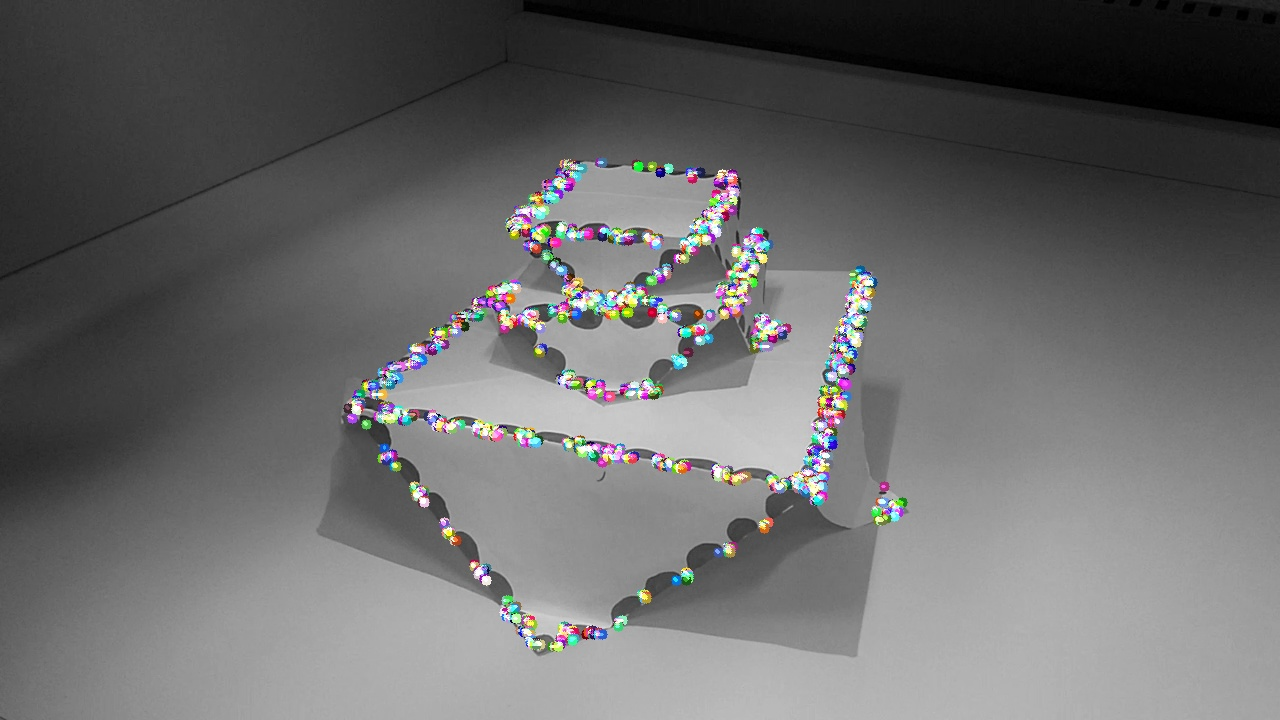
\includegraphics[width=0.9\linewidth]{figs/kpts-Harris.jpg}
	  \caption{Harris}
	\end{subfigure}%
	\begin{subfigure}{0.5\textwidth}
	  \centering
	  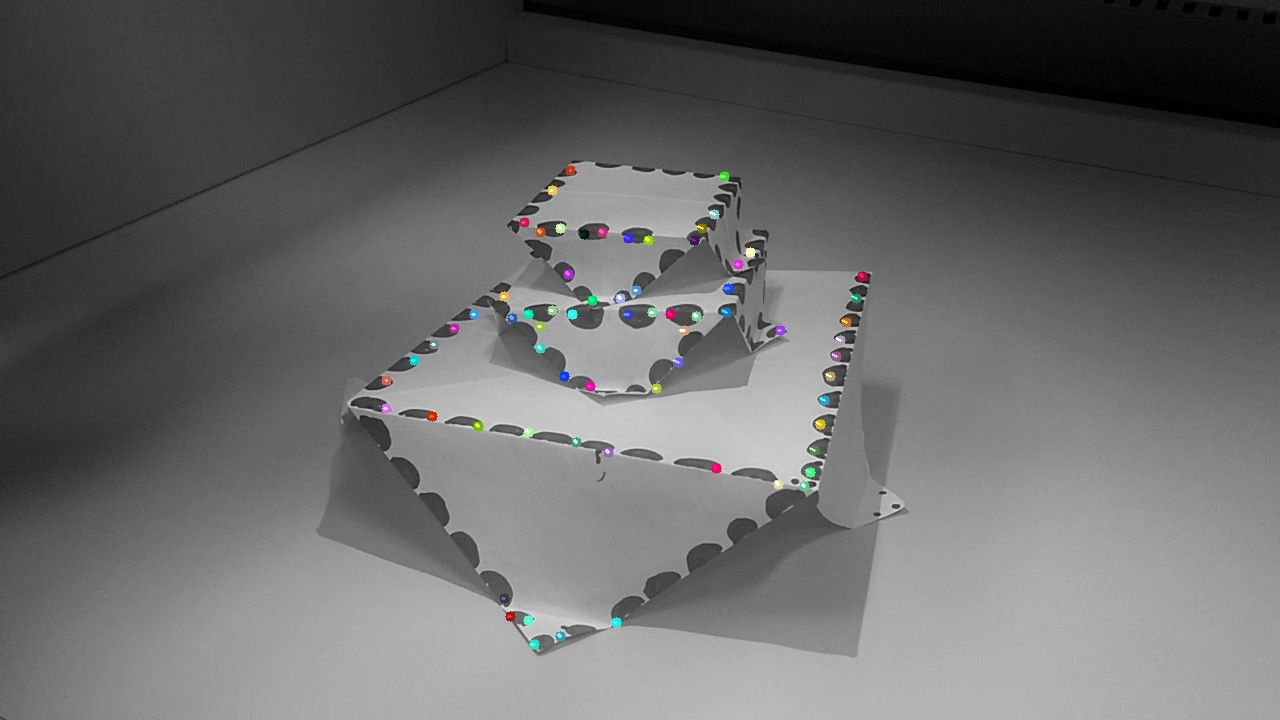
\includegraphics[width=0.9\linewidth]{figs/kpts_Shitomosi.jpg}
	  \caption{Shi-Tomasi}
	\end{subfigure}
	\begin{subfigure}{0.5\textwidth}
        \centering
        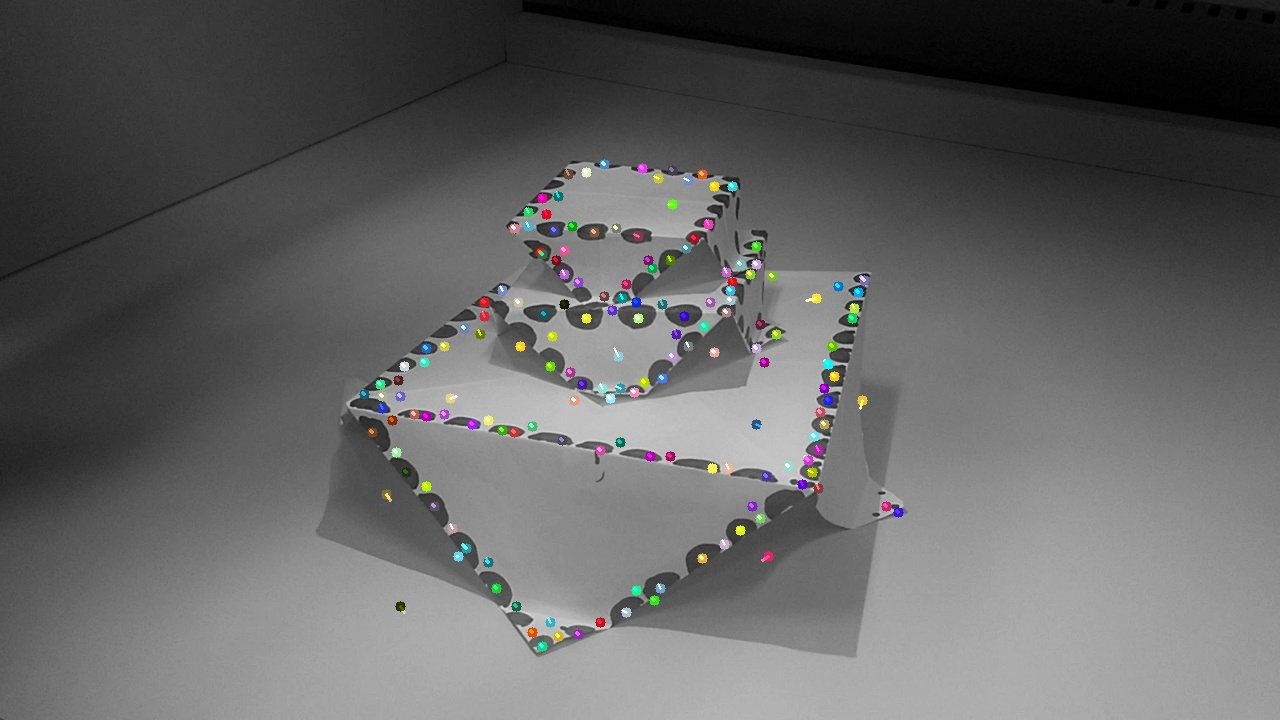
\includegraphics[width=0.9\linewidth]{figs/kpts_Sift.jpg}
        \caption{SIFT}
      \end{subfigure}
       \caption{Comparison of keyppoint detectors}
	\label{fig:comparison-keypoints}
\end{figure}

As can be seen in the figure \ref{fig:comparison-keypoints}, Harris detects a lot of keypoints, most of them are overlapped, Shi-Tomasi detects similar points like Harris but removes the cases of overlap and on the other hand SIFT detects points that at first glance may look desirable but there are cases where these points are in the foreground and not in the object that we want to reconstruct, and this creates noise in the final reconstruction. Thus, we consider to use Harris because it has more points than Shi-Tomasi and all of them are in the object of interest close to the borders.

